\chapter{Isoparametric Elements\index{Elements}}
\label{app:elements}

The base for every Finite Elements computation is its mesh and the elements that are used within that mesh. The element types that can be used depend on the mesh, but also on the dimensionality of the problem (1D, 2D or 3D). In \akantu several isoparametric Lagrangian element types are supported  (and one serendipity element). Each of these types is discussed in more detail below, starting with the 1D-elements all the way to the 3D-elements. For each element type the coordinates of the nodes are given in the isoparametric frame of reference, together with the shape functions (and their derivatives) on these respective nodes. Also all the Gaussian quadrature points within each element are listed (together with the weight that is applied on these points).

%%%%%%%%%% 1D %%%%%%%%%
\section{Isoparametric Elements in 1D\index{Elements!1D}}

In \akantu there are two types of isoparametric elements defined in 1D. These element types are called \code{\_segment\_2} and \code{\_segment\_3}, and are depicted in Figure~\ref{fig:app:elements:1D}.

\begin{figure}[!htb]
\begin{center}
\begin{tabular}{m{0.3\textwidth}m{0.1\textwidth}m{0.3\textwidth}}
\subfloat[\code{\_segment\_2}]{
  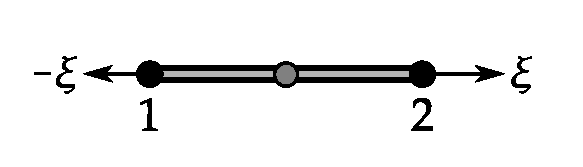
\includegraphics[width=0.3\textwidth]{figures/elements/segment_2}
  \label{fig:appendix:elements:segment2}
} & &
\subfloat[\code{\_segment\_3}]{
  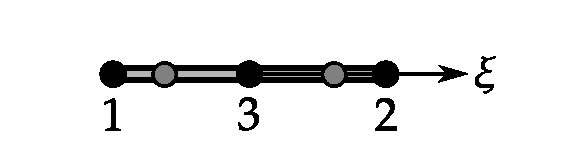
\includegraphics[width=0.3\textwidth]{figures/elements/segment_3}
  \label{fig:appendix:elements:segment3}
} 
\end{tabular}
\end{center}
\caption{Schematic overview of the two 1D element types in \akantu. In each element the node numbering as used in \akantu is indicated and also the quadrature points are highlighted (gray circles). This figure is the same as Figure~\ref{fig:elements:1D} and is repeated here for convience.}
\label{fig:app:elements:1D}
\end{figure}

\subsection{Segment 2\index{Elements!1D!Segment 2}}

\begin{Element}{1D}
 1  &  \inelemone{-1}  &  $\half\left(1-\xi\right)$  &  \inelemone{-\half} \\
\elemline
 2  &  \inelemone{1}   &  $\half\left(1+\xi\right)$  &  \inelemone{\half}  \\
\end{Element}

\begin{QuadPoints}{lc}
Coord. \elemcooroned  &  0  \\
\elemline
Weight  &  2  \\
\end{QuadPoints}

\subsection{Segment 3\index{Elements!1D!Segment 3}}

\begin{Element}{1D}
 1  &  \inelemone{-1}  &  $\half\xi\left(\xi-1\right)$  &  \inelemone{\xi-\half}   \\
\elemline
 2  &  \inelemone{1}   &  $\half\xi\left(\xi+1\right)$  &  \inelemone{\xi+\half}   \\
\elemline
 3  &  \inelemone{0}   &  $1-\xi^{2}$                    &  \inelemone{-2\xi}       \\
\end{Element}

\begin{QuadPoints}{lcc}
Coord. \elemcooroned  &  $-1/\sqrt{3}$  &  $1/\sqrt{3}$  \\
\elemline
Weight  &  1  &  1  \\
\end{QuadPoints}

%%%%%%%%%% 2D %%%%%%%%%
\section{Isoparametric Elements in 2D\index{Elements!2D}}

In \akantu there are four types of isoparametric elements defined in 2D. These element types are called \code{\_triangle\_3} (linear), \code{\_triangle\_6}, \code{\_quadrangle\_4} (both quadratic) and \code{\_quadrangle\_8} (cubic and a serendipity element), and all of  them are depicted in Figure~\ref{fig:app:elements:2D}.

\begin{figure}[!htb]
\begin{center}
\begin{tabular}{m{0.3\textwidth}m{0.1\textwidth}m{0.3\textwidth}}
\subfloat[\code{\_triangle\_3}]{
  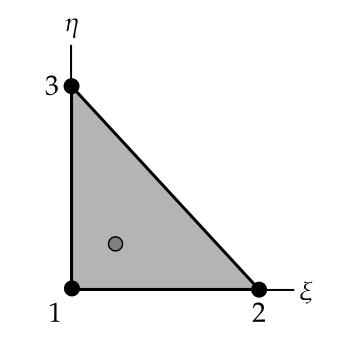
\includegraphics[width=0.3\textwidth]{figures/elements/triangle_3}
  \label{fig:appendix:elements:triangle3}
} & &
\subfloat[\code{\_triangle\_6}]{
  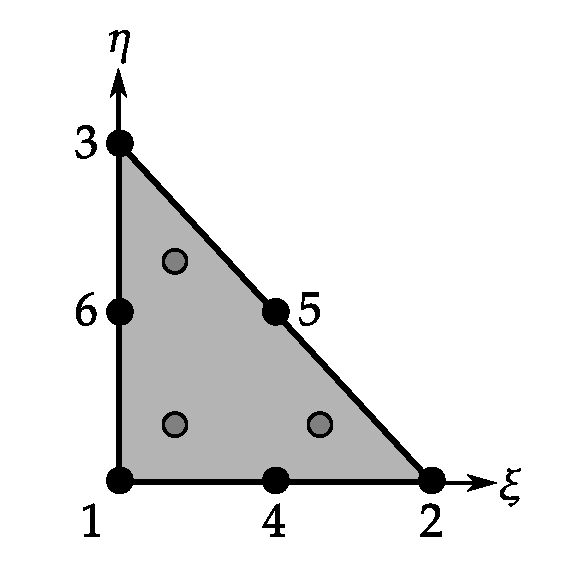
\includegraphics[width=0.3\textwidth]{figures/elements/triangle_6}
  \label{fig:appendix:elements:triangle6}
} \\
\subfloat[\code{\_quadrangle\_4}]{
  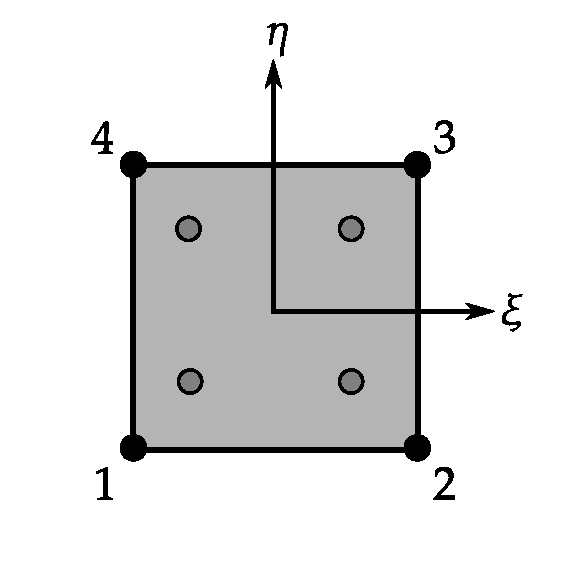
\includegraphics[width=0.3\textwidth]{figures/elements/quadrangle_4}
  \label{fig:appendix:elements:quadrangle4}
} & &
\subfloat[\code{\_quadrangle\_8}]{
  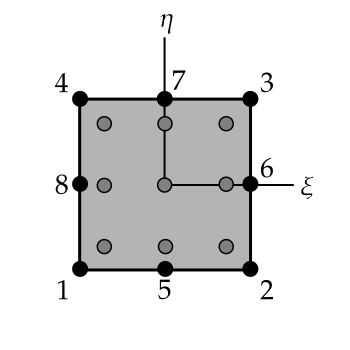
\includegraphics[width=0.3\textwidth]{figures/elements/quadrangle_8}
  \label{fig:appendix:elements:quadrangle8}
} 
\end{tabular}
\end{center}
\caption{A schematic overview of the four 2D element types in \akantu. In each element the node numbering as used in \akantu is indicated and also the quadrature points are highlighted (gray circles). This figure is the same as Figure~\ref{fig:elements:2D} and is repeated here for convience.}
\label{fig:app:elements:2D}
\end{figure}

\clearpage
\subsection{Triangle 3\index{Elements!2D!Triangle 3}}

\begin{Element}{2D}
 1  &  \inelemtwo{0}{0}  &  $1-\xi-\eta$  &  \inelemtwo{-1}{-1}  \\
\elemline
 2  &  \inelemtwo{1}{0}  &  $\xi$         &  \inelemtwo{1}{0}    \\
\elemline
 3  &  \inelemtwo{0}{1}  &  $\eta$        &  \inelemtwo{0}{1}    \\
\end{Element}

\begin{QuadPoints}{lc}
Coord. \elemcoortwod  &  \inquadtwo{\third}{\third}  \\
\elemline
Weight  &  1  \\
\end{QuadPoints}

\subsection{Triangle 6\index{Elements!2D!Triangle 6}}

\begin{Element}{2D}
 1  &  \inelemtwo{0}{0}          &  $-\left(1-\xi-\eta\right)\left(1-2\left(1-\xi-\eta\right)\right)$ & \inelemtwo{1-4\left(1-\xi-\eta\right)}{1-4\left(1-\xi-\eta\right)} \\
\elemline
 2  &  \inelemtwo{1}{0}          &  $-\xi\left(1-2\xi\right)$                                         & \inelemtwo{4\xi-1}{0}                          \\
\elemline
 3  &  \inelemtwo{0}{1}          &  $-\eta\left(1-2\eta\right)$                                       & \inelemtwo{0}{4\eta-1}                   \\
\elemline
 4  &  \inelemtwo{\half}{0}      &  $4\xi\left(1-\xi-\eta\right)$                                     & \inelemtwo{4\left(1-2\xi-\eta\right)}{-4\xi}                      \\
\elemline
 5  &  \inelemtwo{\half}{\half}  &  $4\xi\eta$                                                        & \inelemtwo{4\eta}{4\xi}                       \\
\elemline
 6  &  \inelemtwo{0}{\half}      &  $4\eta\left(1-\xi-\eta\right)$                                    & \inelemtwo{-4\eta}{4\left(1-\xi-2\eta\right)}  \\
\elemline
\end{Element}

\begin{QuadPoints}{lccc}
Coord. \elemcoortwod  &  \inquadtwo{\sixth}{\sixth} & \inquadtwo{\twothird}{\sixth} & \inquadtwo{\sixth}{\twothird} \\
\elemline
Weight & \sixth & \sixth & \sixth \\
\end{QuadPoints}

\subsection{Quadrangle 4\index{Elements!2D!Quadrangle 4}}

\begin{Element}{2D}
 1  &  \inelemtwo{-1}{-1}  &  $\quart\left(1-\xi\right)\left(1-\eta\right)$  &  \inelemtwo{-\quart\left(1-\eta\right)}{-\quart\left(1-\xi\right)} \\
\elemline
 2  &  \inelemtwo{1}{-1}   &  $\quart\left(1+\xi\right)\left(1-\eta\right)$  &  \inelemtwo{\quart\left(1-\eta\right)}{-\quart\left(1-\xi\right)} \\
\elemline
 3  &  \inelemtwo{1}{1}    &  $\quart\left(1+\xi\right)\left(1+\eta\right)$  &  \inelemtwo{\quart\left(1-\eta\right)}{\quart\left(1-\xi\right)}  \\
\elemline
 4  &  \inelemtwo{-1}{1}   &  $\quart\left(1-\xi\right)\left(1+\eta\right)$  &  \inelemtwo{-\quart\left(1-\eta\right)}{\quart\left(1-\xi\right)}  \\
\end{Element}

\begin{QuadPoints}{lcccc}
\elemcoortwod  &  \inquadtwo{-\invsqrtthree}{-\invsqrtthree}  &  \inquadtwo{\invsqrtthree}{-\invsqrtthree}  
               &  \inquadtwo{\invsqrtthree}{\invsqrtthree}    &  \inquadtwo{-\invsqrtthree}{\invsqrtthree} \\ 
\elemline
Weight & 1 & 1 & 1 & 1 \\
\end{QuadPoints}

\clearpage
\subsection{Quadrangle 8\index{Elements!2D!Quadrangle 8}}

\begin{Element}{2D}
 1  &  \inelemtwo{-1}{-1}  &  $\quart\left(1-\xi\right)\left(1-\eta\right)\left(-1-\xi-\eta\right)$ 
                           &  \inelemtwo{\quart\left(1-\eta\right)\left(2\xi+\eta\right)}
                                        {\quart\left(1-\xi\right)\left(\xi+2\eta\right)}  \\
\elemline
 2  &  \inelemtwo{1}{-1}  &  $\quart\left(1+\xi\right)\left(1-\eta\right)\left(-1+\xi-\eta\right)$ 
                          &  \inelemtwo{\quart\left(1-\eta\right)\left(2\xi-\eta\right)}
                                       {-\quart\left(1+\xi\right)\left(\xi-2\eta\right)} \\
\elemline
 3  &  \inelemtwo{1}{1}  &  $\quart\left(1+\xi\right)\left(1+\eta\right)\left(-1+\xi+\eta\right)$ 
                         &  \inelemtwo{\quart\left(1+\eta\right)\left(2\xi+\eta\right)}
                                      {\quart\left(1+\xi\right)\left(\xi+2\eta\right)}  \\
\elemline
 4  &  \inelemtwo{-1}{1}  &  $\quart\left(1-\xi\right)\left(1+\eta\right)\left(-1-\xi+\eta\right)$ 
                          &  \inelemtwo{\quart\left(1+\eta\right)\left(2\xi-\eta\right)}
                                       {-\quart\left(1-\xi\right)\left(\xi-2\eta\right)} \\
\elemline
 5  &  \inelemtwo{0}{-1}  &  $\half\left(1-\xi^{2}\right)\left(1-\eta\right)$ 
                          &  \inelemtwo{-\xi\left(1-\eta\right)}
                                       {-\half\left(1-\xi^{2}\right)}  \\
\elemline
 6  &  \inelemtwo{1}{0}  &  $\half\left(1+\xi\right)\left(1-\eta^{2}\right)$
                         &  \inelemtwo{\half\left(1-\eta^{2}\right)}
                                      {-\eta\left(1+\xi\right)}  \\
\elemline
 7  &  \inelemtwo{0}{1}  &  $\half\left(1-\xi^{2}\right)\left(1+\eta\right)$
                         &  \inelemtwo{-\xi\left(1+\eta\right)}
                                      {\half\left(1-\xi^{2}\right)}  \\
\elemline
 8  & \inelemtwo{-1}{0}  &  $\half\left(1-\xi\right)\left(1-\eta^{2}\right)$
                         &  \inelemtwo{-\half\left(1-\eta^{2}\right)}
                                      {-\eta\left(1-\xi\right)}  \\
\end{Element}

\begin{QuadPoints}{lccccc}
Coord. \elemcoortwod & \inquadtwo{0}{0} & \inquadtwo{\sqrt{\tfrac{3}{5}}}{\sqrt{\tfrac{3}{5}}} & \inquadtwo{-\sqrt{\tfrac{3}{5}}}{\sqrt{\tfrac{3}{5}}} 
                     & \inquadtwo{-\sqrt{\tfrac{3}{5}}}{-\sqrt{\tfrac{3}{5}}} & \inquadtwo{\sqrt{\tfrac{3}{5}}}{-\sqrt{\tfrac{3}{5}}} \\
\elemline
Weight & 64/81 & 25/81 & 25/81 & 25/81 & 25/81 \\
\elemline
Coord. \elemcoortwod & \inquadtwo{0}{\sqrt{\tfrac{3}{5}}} & \inquadtwo{-\sqrt{\tfrac{3}{5}}}{0} 
                     & \inquadtwo{0}{-\sqrt{\tfrac{3}{5}}} & \inquadtwo{\sqrt{\tfrac{3}{5}}}{0} & \\
\elemline
Weight & 40/81 & 40/81 & 40/81 & 40/81 & \\
\end{QuadPoints}

%%%%%%%%%% 3D %%%%%%%%%
\section{Isoparametric Elements in 3D\index{Elements!3D}}

In \akantu there are three types of isoparametric elements defined in 3D. These element types are called \code{\_tetrahedron\_4}, \code{\_tetrahedron\_10} and \code{\_hexahedron\_8}, and all of them are depicted schematically in Figure~\ref{fig:app:elements:3D}. 

\begin{figure}[!htb]
\begin{center}
\begin{tabular}{m{0.3\textwidth}m{0.3\textwidth}m{0.3\textwidth}}
\subfloat[\code{\_tetrahedron\_4}]{
  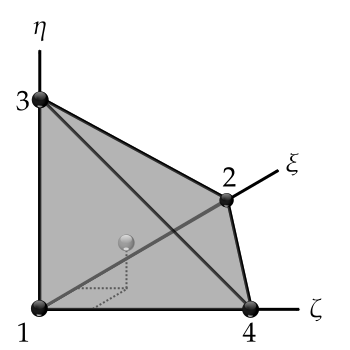
\includegraphics[width=0.3\textwidth]{figures/elements/tetrahedron_4}
  \label{fig:appendix:elements:tetrahedron4}
} &
\subfloat[\code{\_tetrahedron\_10}]{
  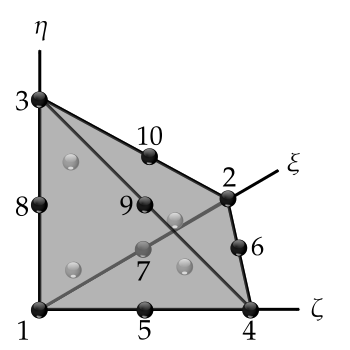
\includegraphics[width=0.3\textwidth]{figures/elements/tetrahedron_10}
  \label{fig:appendix:elements:tetrahedron10}
} &
\subfloat[\code{\_hexahedron\_8}]{
  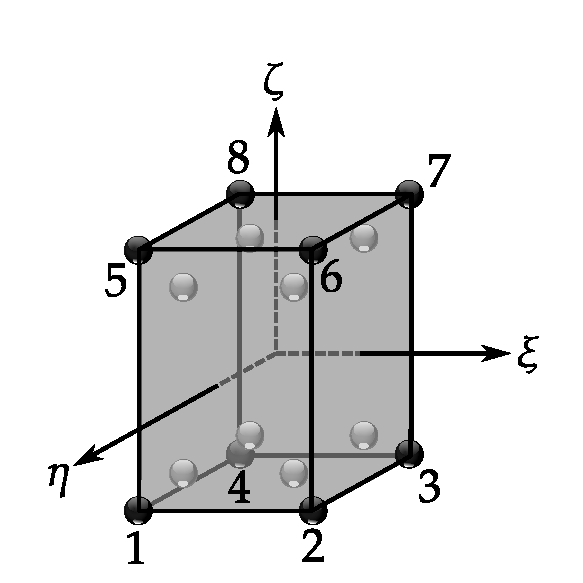
\includegraphics[width=0.3\textwidth]{figures/elements/hexahedron_8}
  \label{fig:appendix:elements:hexahedron8}
} 
\end{tabular}
\caption{A schematic overview of the three supported 3D element types in \akantu. In each element the node numbering as used in \akantu is indicated and also the quadrature points are highlighted (gray spheres). This figure is the same as Figure~\ref{fig:elements:3D} and is repeated here for convience.}
\label{fig:app:elements:3D}
\end{center}
\end{figure}

\clearpage
\subsection{Tetrahedron 4\index{Elements!3D!Tetrahedron 4}}

\begin{Element}{3D}
 1 & \inelemthree{0}{0}{0} & $1-\xi-\eta-\zeta$ & \inelemthree{-1}{-1}{-1} \\
\elemline 
 2 & \inelemthree{1}{0}{0} & $\xi$              & \inelemthree{1}{0}{0} \\
\elemline 
 3 & \inelemthree{0}{1}{0} & $\eta$             & \inelemthree{0}{1}{0} \\
\elemline 
 4 & \inelemthree{0}{0}{1} & $\zeta$            & \inelemthree{0}{0}{1} \\
\end{Element}

\begin{QuadPoints}{lc}
Coord. \elemcoorthreed & \inquadthree{\quart}{\quart}{\quart} \\
\elemline
Weight & \sixth \\
\end{QuadPoints}

\subsection{Tetrahedron 10\index{Elements!3D!Tetrahedron 10}}

\begin{Element}{3D}
  1 & \inelemthree{0}{0}{0} & $\left(1-\xi-\eta-\zeta\right)\left(1-2\xi-2\eta-2\zeta\right)$ 
                            & \inelemthree{4\xi+4\eta+4\zeta-3}{4\xi+4\eta+4\zeta-3}{4\xi+4\eta+4\zeta-3} \\
\elemline
  2 & \inelemthree{1}{0}{0} & $\xi\left(2\xi-1\right)$
                            & \inelemthree{4\xi-1}{0}{0} \\
\elemline
  3 & \inelemthree{0}{1}{0} & $\eta\left(2\eta-1\right)$
                            & \inelemthree{0}{4\eta-1}{0} \\
\elemline
  4 & \inelemthree{0}{0}{1} & $\zeta\left(2\zeta-1\right)$
                            & \inelemthree{0}{0}{4\zeta-1} \\
\elemline
  5 & \inelemthree{\half}{0}{0} & $4\xi\left(1-\xi-\eta-\zeta\right)$
                                & \inelemthree{4-8\xi-4\eta-4\zeta}{-4\xi}{-4\xi} \\
\elemline
  6 & \inelemthree{\half}{\half}{0} & $4\xi\eta$
                                    & \inelemthree{4\eta}{4\xi}{0} \\
\elemline
  7 & \inelemthree{0}{\half}{0} & $4\eta\left(1-\xi-\eta-\zeta\right)$
                                & \inelemthree{-4\eta}{4-4\xi-8\eta-4\zeta}{-4\eta} \\
\elemline
  8 & \inelemthree{0}{0}{\half} & $4\zeta\left(1-\xi-\eta-\zeta\right)$
                                & \inelemthree{-4\zeta}{-4\zeta}{4-4\xi-4\eta-8\zeta} \\
\elemline
  9 & \inelemthree{\half}{0}{\half} & $4\xi\zeta$
                                    & \inelemthree{4\zeta}{0}{4\xi} \\
\elemline
 10 & \inelemthree{0}{\half}{\half} & $4\eta\zeta$
                                    & \inelemthree{0}{4\zeta}{4\eta} \\
\end{Element}

\begin{QuadPoints}{lcc}
Coord. \elemcoorthreed & \inquadthree{\quada}{\quada}{\quada} & \inquadthree{\quadb}{\quada}{\quada} \\
\elemline
Weight & 1/24 & 1/24 \\
\elemline
Coord. \elemcoorthreed & \inquadthree{\quada}{\quadb}{\quada} & \inquadthree{\quada}{\quada}{\quadb} \\
\elemline
Weight & 1/24 & 1/24 \\
\end{QuadPoints}

\clearpage
\subsection{Hexahedron 8\index{Elements!3D!Hexahedron 8}}

\begin{Element}{3D}
 1 & \inelemthree{-1}{-1}{-1} & $\eighth\left(1-\xi\right)\left(1-\eta\right)\left(1-\zeta\right)$ 
                              & \inelemthree{-\eighth\left(1-\eta\right)\left(1-\zeta\right)}
                                            {-\eighth\left(1-\xi\right)\left(1-\zeta\right)}
                                            {-\eighth\left(1-\xi\right)\left(1-\eta\right)} \\
\elemline
 2 & \inelemthree{1}{-1}{-1}  & $\eighth\left(1+\xi\right)\left(1-\eta\right)\left(1-\zeta\right)$ 
                              & \inelemthree{ \eighth\left(1-\eta\right)\left(1-\zeta\right)}
                                            {-\eighth\left(1+\xi\right)\left(1-\zeta\right)}
                                            {-\eighth\left(1+\xi\right)\left(1-\eta\right)} \\
\elemline
 3 & \inelemthree{1}{1}{-1}   & $\eighth\left(1+\xi\right)\left(1+\eta\right)\left(1-\zeta\right)$ 
                              & \inelemthree{ \eighth\left(1+\eta\right)\left(1-\zeta\right)}
                                            { \eighth\left(1+\xi\right)\left(1-\zeta\right)}
                                            {-\eighth\left(1+\xi\right)\left(1+\eta\right)} \\
\elemline
 4 & \inelemthree{-1}{1}{-1}  & $\eighth\left(1-\xi\right)\left(1+\eta\right)\left(1-\zeta\right)$ 
                              & \inelemthree{-\eighth\left(1+\eta\right)\left(1-\zeta\right)}
                                            { \eighth\left(1-\xi\right)\left(1-\zeta\right)}
                                            {-\eighth\left(1-\xi\right)\left(1+\eta\right)} \\
\elemline
 5 & \inelemthree{-1}{-1}{1}  & $\eighth\left(1-\xi\right)\left(1-\eta\right)\left(1+\zeta\right)$ 
                              & \inelemthree{-\eighth\left(1-\eta\right)\left(1+\zeta\right)}
                                            {-\eighth\left(1-\xi\right)\left(1+\zeta\right)}
                                            { \eighth\left(1-\xi\right)\left(1-\eta\right)} \\
\elemline
 6 & \inelemthree{1}{-1}{1}   & $\eighth\left(1+\xi\right)\left(1-\eta\right)\left(1+\zeta\right)$ 
                              & \inelemthree{ \eighth\left(1-\eta\right)\left(1+\zeta\right)}
                                            {-\eighth\left(1+\xi\right)\left(1+\zeta\right)}
                                            { \eighth\left(1+\xi\right)\left(1-\eta\right)} \\
\elemline
 7 & \inelemthree{1}{1}{1}    & $\eighth\left(1+\xi\right)\left(1+\eta\right)\left(1+\zeta\right)$ 
                              & \inelemthree{ \eighth\left(1+\eta\right)\left(1+\zeta\right)}
                                            { \eighth\left(1+\xi\right)\left(1+\zeta\right)}
                                            { \eighth\left(1+\xi\right)\left(1+\eta\right)} \\
\elemline
 8 & \inelemthree{-1}{1}{1}   & $\eighth\left(1-\xi\right)\left(1+\eta\right)\left(1+\zeta\right)$ 
                              & \inelemthree{-\eighth\left(1+\eta\right)\left(1+\zeta\right)}
                                            { \eighth\left(1-\xi\right)\left(1+\zeta\right)}
                                            { \eighth\left(1-\xi\right)\left(1+\eta\right)} \\
\end{Element}

\begin{QuadPoints}{lcccc}
\elemcoortwod  &  \inquadthree{-\invsqrtthree}{-\invsqrtthree}{-\invsqrtthree}  &  \inquadthree{\invsqrtthree}{-\invsqrtthree}{-\invsqrtthree}  
               &  \inquadthree{\invsqrtthree}{\invsqrtthree}{-\invsqrtthree}    &  \inquadthree{-\invsqrtthree}{\invsqrtthree}{-\invsqrtthree} \\ 
\elemline
Weight & 1 & 1 & 1 & 1 \\
\elemline
\elemcoortwod  &  \inquadthree{-\invsqrtthree}{-\invsqrtthree}{\invsqrtthree}   &  \inquadthree{\invsqrtthree}{-\invsqrtthree}{\invsqrtthree}  
               &  \inquadthree{\invsqrtthree}{\invsqrtthree}{\invsqrtthree}     &  \inquadthree{-\invsqrtthree}{\invsqrtthree}{\invsqrtthree} \\ 
\elemline
Weight & 1 & 1 & 1 & 1 \\
\end{QuadPoints}


%%% Local Variables: 
%%% mode: latex
%%% TeX-master: "manual"
%%% End: 
